\documentclass{article}
\usepackage[utf8]{inputenc}
\usepackage{amsfonts}
\usepackage{tikz}
\usepackage{natbib}
\usepackage{graphicx}
\usepackage{url}

\newcommand{\Z}{\mathbb{Z}}
\newcommand{\R}{\mathbb{R}}
\newcommand{\C}{\mathbb{C}}
\newcommand{\CP}{\hat{\mathbb{C}}}

\title{Project Definitions}
\author{Connor Riley }
\date{September 2015}

\begin{document}
\maketitle

\section{Definitions}
 \subsection{Graphs}
  A \textbf{graph} is an ordered pair $G=(V,E)$ which represents a set of objects where some of these objects are linked. In the denotation $G=(V,E)$, $V$ stands for the vertexes or objects, and $E$ stands for the edges or links. Edges in a graph can be directed or undirected, however, we will focus on undirected edges in our application.

 \subsubsection{Components}
  A component or \textbf{connected component} of a graph is a subgraph in which any two vertices are connected to each other by a path which is connected to no additional vertices in the supergraph.

 \subsubsection{Loops}
  A \textbf{loop} is when a vertex has an edge connecting it to itself. \citep{NIST:self-loop}
  \begin{center}
	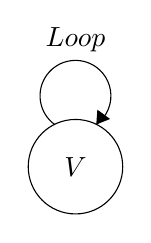
\begin{tikzpicture}[scale=0.2]\tikzstyle{every node}+=[inner sep=0pt]
	  \draw [black] (25.7,-24.2) circle (3);
	  \draw (25.7,-24.2) node {$V$};
      \draw [black] (24.377,-21.52) arc (234:-54:2.25);
      \draw (25.7,-16.95) node [above] {$Loop$};
      \fill [black] (27.02,-21.52) -- (27.9,-21.17) -- (27.09,-20.58);
    \end{tikzpicture}
  \end{center}

 \subsubsection{Multiple Edges}
  A graph with multiple edges is one which has two or more edges connect the same two vertices.
  \begin{center}
	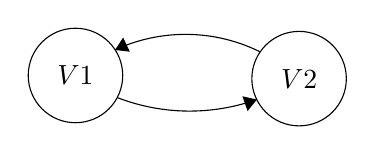
\begin{tikzpicture}[scale=0.2]\tikzstyle{every node}+=[inner sep=0pt]
	  \draw [black] (25.7,-24.2) circle (3);
	  \draw (25.7,-24.2) node {$V1$};
	  \draw [black] (39.9,-24.4) circle (3);
	  \draw (39.9,-24.4) node {$V2$};
	  \draw [black] (37.217,-25.726) arc (-70.44515:-111.16871:12.75);
	  \fill [black] (37.22,-25.73) -- (36.3,-25.52) -- (36.63,-26.46);
	  \draw [black] (28.21,-22.575) arc (114.84766:63.53848:10.656);
	  \fill [black] (28.21,-22.58) -- (29.15,-22.69) -- (28.73,-21.79);
	\end{tikzpicture}
  \end{center}

 \subsection{Types of Graphs}
 \subsubsection{Connected Graphs}
  A graph is \textbf{connected} when there is a path between every pair of vertices. 
  In a connected graph every vertex is reachable. A graph with just one vertex is connected~\citep{mathworld:ConnectedGraphs}.

 \subsubsection{Simple Graphs}
  A \textbf{simple graph} is an unweighted, undirected graph, containing no loops or multiple edges. 
  A simple graph may either be connected or disconnected~\citep{mathworld:SimpleGraphs}.

  \subsubsection{Planar Graphs}
  A \textbf{planar graph} is one that can be embedded in the plane. 
  In other words, the graph can be drawn on the plane in such a way that its edges intersect only at their endpoints (no edges cross each other)~\citep{mathworld:PlanarGraph}.
  \begin{itemize}
	\item A triangulation, also referred to as a maximal planar graph, is a planar graph in which there is no way to add another edge and have the graph continue to be planar. 
	In practice these means that each face is bounded by three edges~\citep{mathworld:Triangulation}.
  \end{itemize}

 \subsection{Embedding}
  An \textbf{embedding} of a graph $G$ on a surface $\Sigma$ is a representation of $G$ on $\Sigma$ in which points of $\Sigma$ are associated to vertices and simple arcs are associated to edges in such a way that:
  \begin{itemize}
	\item The endpoints of the arc associated to the edge $e$ are the points associated to the end vertices of $e$.
	\item No arcs include points associated with other vertices.
	\item Two arcs never intersect at a point which is interior to either of the arcs.
  \end{itemize}

  \subsubsection{Straight-Line Embedding}
  A \textbf{straight-line embedding} is a embedding of a planar graph in which all arcs are straight.

 \subsection{Euler's Formula}
  Euler's formula states that if a finite, connected, planar graph is drawn in the plane without any edge intersections, and $v$ is the number of vertices, $e$ is the number of edges and $f$ is the number of faces (including the outer region), then: 
  \begin{equation} 
	v-e+f=2
  \end{equation}

  If $c$ is the number of components in a graph, then a more general form of Euler's formula is:
  \begin{equation} 
	v-e+f= 1 + c
  \end{equation}

 \subsection{Circle Packing}
  We say that two circles drawn in a plane kiss (or osculate) when they intersect in exactly one point. 
  A \textbf{circle packing} is a graph formed by a set of circles which have no overlapping interiors where each circle kisses its surrounding circles. 
  Formally, a circle packing is a connected collection of circles whose interiors are disjoint. 
  The \textbf{intersection graph} of a circle packing is the graph having a vertex for each circle and an edge for every pair of circles that are tangent. 
  If the circle packing is on the plane or the sphere, then its intersection graph is called a \textbf{coin graph}. 
  Coin graphs are always connected, simple and planar. 

    Common geometric settings for circle packing are the $euclidean$ $plane$, $the$ $sphere$ and the $hyperbolic$ $plane$. Each pair of circles in a packing forms a tangent pair, and the empty space between each $triple$ forms a $interstice$. A $flower$ is the next level of structure, which consists of a central circle and some number of $petal$ circles. The number of petals defines the $degree$ of the central circle. A condition that we will enforce on all circle packings is that every circle must have a flower. This condition is a $local$ $planarity$ condition. \citep{introCirlceacking}
    \subsubsection{Koebe Representation Theorem}
    Given any planar graph $G$ with vertex set $V(G) = \{v_1, ... v_n \}$ and edge set $E(G)$, we can find a packing of n (not necessarily congruent) circular discs $C= \{C_1,... C_n\}$ in the plane with the property that $C_i$ and $C_j$ touch each other if and only if $v_i v_j \epsilon E(G)$ for $1 \le i \le n$. \citep{combinatorialGeometry}
    \subsubsection{Liftings}
    \subsubsection{Stereographic Projections}
    A \textbf{sterographic projection} is a bijective mapping that projects a sphere onto a plane.
     The projection is defined on the entire sphere except for the projection point. 
    As the mapping is bijective there exists an inverse mapping from the plane to the sphere.

    \subsubsection{Mobius Transformations}
    A \textbf{M\"{o}bius Transformation} of a plane can be obtained by performing the stereographic projection of the plane onto a sphere, then rotating or moving the sphere and then performing the sterographic projection back onto the plane. 
    Formally, a M\"{o}bius Transformation is a rational function defined on the extended complex plane $\CP = \C\cup\{\infty\}$ of the form:
    \begin{equation} 
    	f(z) = \frac{az+b}{cz+d}
    \end{equation}
    where $z\in\CP$ is a complex variable and $a,b,c,d\in\CP$ are complex numbers such that $ad - bc$ $\neq$ $0$.

 \subsection{Dual Graph}
  The \textbf{dual graph} of a plane graph $G$ is a graph that has a vertex for each face of $G$. 
  The dual graph has an edge whenever two faces of $G$ are separated from each other by an edge. 
  Thus each edge $e$ of $G$ has a corresponding dual edge, the edge that connects the two faces on either side of $e$. 

  \subsubsection{Dual Packing}
  The \textbf{dual packing} is the circle packing of the dual graph. 
  In this packing, each circle passes through the points where the original circles kiss. 
  The dual packing does not form a triangulation whereas the original circle packing does.

\section{Data Structures}
 \subsection{Half Edge}
  Also called a doubly-connected edge list, the \textbf{half edge} data structure associates two directed half edges to each edge on the graph. 
  Each half edge stores a vertex, a face, the next half edge, the previous half edge and the twin, which is the half edge going in the other direction. 
  Half edges are typically directed counter clockwise with respect to the face they define.

\bibliographystyle{plain}
\bibliography{references}
\end{document}